\documentclass[12pt,fleqn]{article}
\setlength{\parindent}{0pt}
\usepackage{graphicx}
\usepackage{cancel}
\usepackage{listings}
\usepackage[latin5]{inputenc}
\usepackage{color}
\setlength{\parskip}{8pt}
\setlength{\parsep}{0pt}
\setlength{\headsep}{0pt}
\setlength{\topskip}{0pt}
\setlength{\topmargin}{0pt}
\setlength{\topsep}{0pt}
\setlength{\partopsep}{0pt}
\setlength{\mathindent}{0cm}

\begin{document}
Ders 23

Akis (Flux)

Aslinda akis cizgisel entegrallerin degisik bir seklidir. Diyelim ki $C$
egrisi ve $\vec{F}$ vektor alani var, o zaman $C$ uzerinden $\vec{F}$'in
akisi 

\[ \int_C \vec{F} \cdot \hat{n} \ ds \]

olarak gosterilir. Simdi bu entegral icindeki ogelerin ne oldugunu tarif
edelim. 

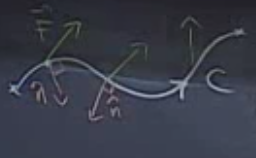
\includegraphics[height=3cm]{23_1.png}

$\hat{n}$ = $C$ egrisine dik olan birim normal vektordur, $\vec{T}$'ye 90
derece saat yonunde diktir. Saat yonunde dedik cunku mesela ustteki resimde
en soldaki $\hat{n}$ yukari da isaret ediyor olabilirdi, onu degil, asagi
dogru gideni sectik.

Entegral neyi hesaplar? Egri uzerindeki her noktada, vektor alani ile ayni
egrinin normalleri ile yapilan carpimlarin toplamini. Yani $C$'yi en ufak
parcalar $\Delta s$'lere ayirinca 

\[ Akis = \lim_{\Delta s \to 0} 
\bigg( \sum \vec{F} \cdot \hat{n} \ \Delta s \bigg) \]

Bu kavrami daha once hesapladigimiz ``yapilan is'' karsilastirmak
gerekirse

\[ Is = \int_C \vec{F} \cdot d\vec{r} = \int_C \vec{F} \cdot \vec{T} \ ds \]

Isi hesaplarken her noktada $\vec{F}$'in egri $C$'nin tegetine yansimasini
hesapliyorum. 

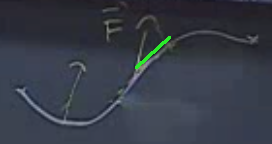
\includegraphics[height=2cm]{23_2.png}

Yani egri uzerinde hareket ederken ``$\vec{F}$ ile ne kadar birlikte, ne
kadar ona ters sekilde'' hareket edildiginin hesabini yapilan isi veriyor. 

Kiyasla akis hesabi, egri uzerinde hareket ederken $\vec{F}$'in egrinin
``ne kadar icinden gectiginin'' hesabi. Ruzgarli bir havada bir yolda
yuruyorum, akis ruzgarin bana ne kadar yandan carptigini gosteriyor. Akis
hesabi bu carpis saga dogru olunca onu pozitif, saga dogru olunca onu
negatif olarak hesaplar. 

Yani yapilan is $\vec{F}$'in tegetsel bilesenlerinin, yansimasinin toplami
ise, akis $\vec{F}$'in normal bilesenlerinin toplamidir. Bu ufak fark
haricinde bu iki hesap birbirinin aynisidir. Yani fiziksel anlamlari cok
farkli olabilir fakat matematiksel anlamda ikisi de bir cizgisel entegral,
ve hesaplanislari, tanimlari birbirine benzer. 

Anlatim baglaminda is hesabi icin $\vec{F}$'i bir kuvvet alani olarak gormek
anlatimi rahatlatiyor ($\vec{F}$ baska bir sey de olabilir). Akis
baglaminda $\vec{F}$'i bir hiz alani (velocity field) olarak gormek
benzer bir rahatlik sagliyor. 

Bir siviyi dusunursek, akis birim zamanda $C$'nin icinden ne kadar sivinin
gectigini gosterir. Diyelim ki boyle bir alan alttaki gibi

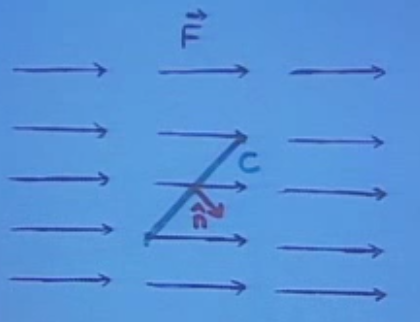
\includegraphics[height=4cm]{23_3.png}

Alan bir sabit alan, ama herhangi bir alana yeterince zoom edersek, o zaman
goruntusunun ustteki gibi olacagini dusunebiliriz. Simdi bu alan icinde
$C$'nin bir parcasi $\Delta s$'i hayal edelim, ve birim zaman icinde bu
alanin parcamiz icinden gecisini hayal edelim [hoca iki saydam ustuste
getirerek o parcayi oraya koydu, alanin gecisini gostermek icin parcayi
sola hareket ettiriyor, yani alanin saga dogru gecisini goruyoruz].

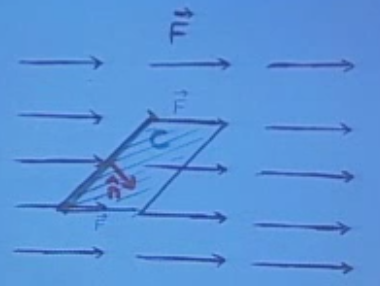
\includegraphics[height=4cm]{23_4.png}

Bu gecis birim zaman icinde ustteki gibi bir sekil olusturacaktir, bu
sekil bir paralelogramdir. 



















\end{document}
